\section{\ix Design Approach}
\label{sec:design}

The first three requirements of \S\ref{sec:motivation:challenges} --
high packet rate, microsecond latency, and connection scalability--
are not unique to web-scale applications.  These requirements have
been addressed in the design of middleboxes such as firewalls,
load-balancers, and software
routers~\cite{routebricks,click};
by integrating the networking stack and the application into a single
\emph{dataplane}. The two remaining requirements -- resource
elasticity and protection -- are not addressed in middleboxes because
they are single-purpose systems, not exposed directly to users.

Dataplanes differ from traditional OS designs in two fundamental
ways. First, they are designed to \emph{run each packet to
  completion}. All network protocol and application processing for a
packet is done before moving on to the next packet.  In contrast, a
commodity OS decouples protocol processing from the application itself
in order to provide scheduling and flow control flexibility.  For
example, a commodity OS relies on device and soft interrupts to
context switch from application to protocol processing. Similarly, the
kernel's networking stack will generate a TCP \texttt{ACK} and slide
its receive window even when the application is not consuming data, up
to an extent. Second, dataplanes are designed to operate in a
\emph{flow-consistent, coherence-free} manner.  Network flows are
distributed into distinct queues via receive-side scaling
(RSS)~\cite{url:rss} and the common case packet processing requires no
synchronization or coherence traffic between cores.

Building upon the lessons from middleboxes, we design \ix to answer
the following question: {\it \ana{how} can the dataplane architecture be
  efficiently extended to support untrusted, event-driven applications
  and satisfy simultaneously the five requirements of
  \S\ref{sec:motivation:challenges}?}  The answer relies on the
following key design principles:

\christos{this list must be aligned with the list in 2.2. Ie we should
  be able to explain how each approach helps with the
  requirements. This is critical}

\myparagraph{Separation and protection of control and data plane:} 
Our design separates the control function of the kernel, responsible
for resource configuration, provisioning, scheduling, and monitoring,
from the dataplane, which runs the networking stack and application
logic.  Like a conventional OS, the control plane multiplexes and
schedules resources among dataplanes, but in a coarse-grained manner
in space and time: entire cores are dedicated to dataplanes,
memory is allocated at large page granularity, and
network device queues are partitioned among dataplanes.
Moreover, the control plane plays a coordination role in elatistically
adjusting the allocation of these resources between dataplanes.

The separation of control and data plane allows us to consider radically
different I/O APIs and implementations in the dataplane, while
permitting other OS functionality (e.g., file system
support) to be passed through to the control plane for compatibilility.
Similar to the
Exokernel~\cite{DBLP:conf/sosp/EnglerKO95}, each data plane runs a
single application in a single address space. However,
we use modern virtualization hardware and Dune~\cite{dune} to
safely and efficiently expose privileged hardware features directly to
dataplanes. As a result, dataplanes have capabilities similar to
virtualization guest OSes; they can manage
their own address translations (on top of the address space provided by
the control plane) and can prevent application logic from corrupting
the network stack through use of privilege ring hardware.

\christos{we should bring up HW virtualization here, likely as a
  independent part of the approach or merged with the one above. It is
  a big part of the protection story. The discussion on CP/DP
  seperation must be linked to elasticity too}


\myparagraph{Run to completion with adaptive batching:} Our dataplane
runs to completion all pipeline stages needed to receive and transmit a
packet, interleaving protocol processing (kernel mode) and application
logic (user mode) at fixed transition points. Hence, there is no need for intermediate
buffering between pipeline stages or between the application logic and
the TCP/IP stack. Run to completion is beneficial for both throughput
and latency because it improves d-cache behavior (each processing stage
is likely to reuse many of the same cache lines).

Our use of run to completion is inspired by work on receive livelock
~\cite{receive-livelock}, which uses a similar approach
to guaruntee forward progress during periods of unmanagable recieve packet load.
By contrast, we apply run to completion in all situations, allowing
us to use polling and avoid interrupt overhead in the common case. However,
we still rely on interrupts as a fallback to regain control,
for example, if the application becomes unresponsive.

We also make extensive use of batching. Batching can increase throughput because it
improves instruction locality as well as the effectiveness of hardware
prefetching and branch prediction. When applied correctly, batching can also
decrease latency because these same efficiencies can reduce head-of-line blocking.
Batching has been shown to improve performance when applied at the system call
boundary~\cite{DBLP:conf/osdi/HanMCR12, DBLP:conf/osdi/SoaresS10}. Similarly,
mTCP~\cite{jeong2014mtcp}, a user-level network stack, applies batching
at the API level and at the hardware queue level.
We improves upon previous batching systems in two ways.
Firstly, we batch at each processing stage in our pipeline. Secondly, we
minimize the impact on latency and maximize efficiency by using batching
\emph{adaptively} as follows: (i) we never wait to batch requests and batching
only occurs in the presence of congestion; (ii) we set an upper bound on
the number of batched packets to avoid exceeding the size of the data cache.

The combination of bounded batch sizes and run to completion means that
queues for incoming packets can build up only at the NIC edge, before
packets are processed by the dataplane. \ana{Emphasize that we are not
  wasting resources on packets that might have to be dropped; drop
  early at the NIC if can't handle.  Citation for Mogul and
  Ramakrishnan could go here.} The networking stack sends
acknowledgments to peers only as fast as the application can process
them. Any slowdown in the application-processing rate quickly leads to
shrinking windows in peers. The dataplane also monitors queue depths
at the NIC edge and signals the control plane to allocate additional
resources for the dataplane (more hardware threads, increased clock
frequency), notify peers explicitly about congestion (e.g., via
ECN~\cite{ramakrishnan2001addition}), and make policy decisions for
congestion management (e.g., via
RED~\cite{DBLP:journals/ton/FloydJ93}).

\begin{figure}
\begin{centering}
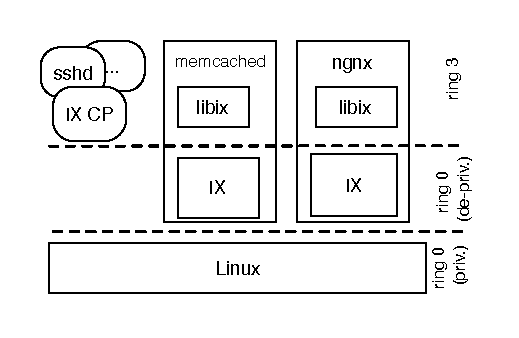
\includegraphics{figs/cp-dp.eps}
\centering\caption{Protection and separation in \ix.}
\label{fig:cp-dp}
\end{centering}
\end{figure}



\myparagraph{Native zero-copy API with explicit flow control:} We do
not expose or emulate the POSIX API for networking.  Instead, the
dataplane and the application communicate asynchronously with each
other via messages stored in
memory~\cite{DBLP:conf/osdi/HanMCR12,DBLP:journals/cacm/Rizzo12}.  The API meets the
commutativity rule~\cite{DBLP:conf/sosp/ClementsKZMK13} and allows for
a true zero-copy operation in both directions. The dataplane and
application cooperatively manage the message buffer pool. Incoming
packets are mapped read-only into the application, which may hold onto
message buffers and return them to the dataplane at a later point.
The application sends to the dataplane scatter/gather lists of memory
locations for transmission but, since contents are not copied, the
application must keep the content immutable until the peer
acknowledges reception. The kernel implements all flow control
mechanisms and may trim transmission requests that exceed the
available size of the sliding window.  Essentially, the API directly,
but safely, exposes flow control to applications.


\myparagraph{Flow consistent, coherence-free processing:} We use
multi-queue NICs with RSS support to provide flow-consistent hashing
of incoming traffic to distinct hardware queues. \data{Each queue is served
by a single hardware thread}{XXX REDO} all the way to the application layer,
eliminating the need for synchronization and cache coherence traffic
between cores. Similarly, memory management is organized in distinct
pools for each hardware thread. The absence of a socket layer
eliminates the issue of the shared file descriptor namespace in
multithreaded
applications~\cite{DBLP:conf/sosp/ClementsKZMK13}. Hence, our design
scales well with the increasing number of cores in modern servers. Our
approach does not restrict the memory model for
applications. Application logic can take advantage of coherent, shared
memory to exchange information and synchronize between cores.




